\documentclass[%
11pt,%
%oneside,%
twoside,%
%twocolumn,%
titlepage,%
%fleqn,%
%a4page,%
german,%
headsepline%
]{scrartcl}

\usepackage{lastpage}
\usepackage{geometry}
\usepackage{graphicx}
\usepackage[utf8]{inputenc}
\usepackage[ngerman]{babel}
\usepackage{lscape}
\usepackage[framemethod=TikZ]{mdframed}
\usepackage[most]{tcolorbox}
\usepackage{mymath}
\usepackage{units}
\usepackage{nicefrac}
\usepackage{pgf,tikz}
\usepackage{pgfplots}
\pgfplotsset{width=10cm,compat=1.9}

\usetikzlibrary{arrows}
\usetikzlibrary{calc, shapes, backgrounds}
\usepackage{colortbl}
\usepackage{hhline}
\usepackage{multirow}
\usepackage[extendedchars]{grffile}
\usepackage{caption}
\usepackage{multicol,calc}
\usepackage{blindtext}
\usepackage{pdfpages}
\usepackage{hyperref}
\usepackage{wrapfig}
\usepackage{booktabs}

\usepackage{marginnote}
\usepackage{qrcode}
\qrset{height=9ex}

%Gothic-Font
\usepackage{oldgerm}
\usepackage{pifont}
\usepackage{yfonts}

% footnote-symbols
\usepackage[symbol]{footmisc}
\renewcommand{\thefootnote}{\fnsymbol{footnote}}

% Command, um Tabellen-Spalten anzupassen
\newcommand{\spaltenheight}{\rule{0mm}{3ex}}
\newcommand{\spaltenwidth}{\rule{3cm}{0mm}}
\newcommand{\spaltensep}{\\[1ex]}
\doublerulesepcolor{white}

\usepackage{fontawesome} % FontAwesome, falls du ein Augensymbol brauchst
\definecolor{lightgray}{rgb}{0.7, 0.7, 0.7}
\newcommand{\faEyeLightGray}{\textcolor{lightgray}{\faEye}} % Custom command for the gray eye icon


% Pagestyle/Layout
\setlength{\parindent}{0pt} \setlength{\parskip}{1em}

\pagestyle{headings} % gemachte Einstellungen anwenden

% Farbig umrahmte Umgebung Satz 
 \definecolor{myblizzardblue}{HTML}{87CEEB}

\newcounter{satzz}[section]\setcounter{satzz}{0}
\renewcommand{\thesatz}{\arabic{section}.\arabic{satzz}}

\newenvironment{csatz}[1][]{%
    \refstepcounter{satzz}
 
    \ifstrempty{#1}%
    % if condition (without title)
    {\mdfsetup{%
        frametitle={%
            \tikz[baseline=(current bounding box.east),outer sep=0pt]
            \node[anchor=east,rectangle,fill=myblizzardblue]
            {\strut Satz~\thesatz};}
        }%
    % else condition (with title)
    }{\mdfsetup{%
        frametitle={%
            \tikz[baseline=(current bounding box.east),outer sep=0pt]
            \node[anchor=east,rectangle,fill=myblizzardblue]
            {\strut Satz~\thesatz:~#1};}%
        }%
    }%
% for both conditions
    \mdfsetup{%
        innertopmargin=10pt,linecolor=myblizzardblue,%
        backgroundcolor=whitesmoke,%
        linewidth=2pt,topline=true,%
        frametitleaboveskip=\dimexpr-\ht\strutbox\relax%
    }
 
\begin{mdframed}[]\relax}{%
\end{mdframed}}

% Farbig umrahmte Umgebung Theorem
\definecolor{mygraphblue}{HTML}{84B7E1}
\definecolor{whitesmoke}{HTML}{F5F5F5}

\newcounter{theo}[section]\setcounter{theo}{0}
\renewcommand{\thetheo}{\arabic{section}.\arabic{theo}}

\newenvironment{ctheo}[1][]{%
    \refstepcounter{theo}
 
    \ifstrempty{#1}%
    % if condition (without title)
    {\mdfsetup{%
        frametitle={%
            \tikz[baseline=(current bounding box.east),outer sep=0pt]
            \node[anchor=east,rectangle,fill=mygraphblue]
            {\strut Theorem~\thetheo};}
        }%
    % else condition (with title)
    }{\mdfsetup{%
        frametitle={%
            \tikz[baseline=(current bounding box.east),outer sep=0pt]
            \node[anchor=east,rectangle,fill=mygraphblue]
            {\strut Theorem~\thetheo:~#1};}%
        }%
    }%
% for both conditions
    \mdfsetup{%
        innertopmargin=10pt,linecolor=mygraphblue,%
        backgroundcolor=whitesmoke,%
        linewidth=2pt,topline=true,%
        frametitleaboveskip=\dimexpr-\ht\strutbox\relax%
    }
 
\begin{mdframed}[]\relax}{%
\end{mdframed}}

% Farbig umrahmte Umgebung Definition
 \definecolor{emerald}{HTML}{50C878}

\newcounter{deff}[section]\setcounter{deff}{0}
\renewcommand{\thedeff}{\arabic{section}.\arabic{deff}}

\newenvironment{cdef}[1][]{%
    \refstepcounter{deff}
 
    \ifstrempty{#1}%
    % if condition (without title)
    {\mdfsetup{%
        frametitle={%
            \tikz[baseline=(current bounding box.east),outer sep=0pt]
            \node[anchor=east,rectangle,fill=emerald]
            {\strut Definition~\thedeff};}
        }%
    % else condition (with title)
    }{\mdfsetup{%
        frametitle={%
            \tikz[baseline=(current bounding box.east),outer sep=0pt]
            \node[anchor=east,rectangle,fill=emerald]
            {\strut Definition~\thedeff:~#1};}%
        }%
    }%
% for both conditions
    \mdfsetup{%
        innertopmargin=10pt,linecolor=emerald,%
        backgroundcolor=whitesmoke,%
        linewidth=2pt,topline=true,%
        frametitleaboveskip=\dimexpr-\ht\strutbox\relax%
    }
 
\begin{mdframed}[]\relax}{%
\end{mdframed}}

%\newtheorem{uebthm}{Übung}[section]
% Umgebung lsg mit dynamischer Referenzierung und Label
\newcommand{\concatueb}[1]{ueb:#1}% Definition für concatueb
\newcommand{\concatlsg}[1]{lsg:#1}% Definition für concatlsg

\newcounter{uebcounter}[section]
\renewcommand{\theuebcounter}{\thesection.\arabic{uebcounter}}  % Zählerformat: Abschnitt.Übung

% Definition einer Übungsumgebung mit dynamischen Labels
\newcommand{\uebh}[2]{%
 \refstepcounter{uebcounter} % Zählt den Übungscounter hoch
 \par\noindent\textbf{Übung \theuebcounter:}\label{\concatueb{#1}} % Label im Format "ueb:1"
    #2
    \hfill\hyperref[\concatlsg{#1}]{\faEyeLightGray}
    \vspace{\parskip}
}

\newenvironment{lsg}[1]{%
    \par\noindent\textbf{Notizen zu Übung \ref{\concatueb{#1}}.}%
    \label{\concatlsg{#1}}
}{%
    \par%
}

\newenvironment{uebenv}[1]{%
    \refstepcounter{uebcounter}
    \par\noindent\textbf{Übung \theuebcounter.}%
    \label{\concatueb{#1}}\hfill\hyperref[\concatlsg{#1}]{\faEyeLightGray}\par
}{%
    \par
}

\newcommand{\definition}[1]{\colorbox{emerald}{#1}}

\setlength{\parindent}{0pt}

\subject{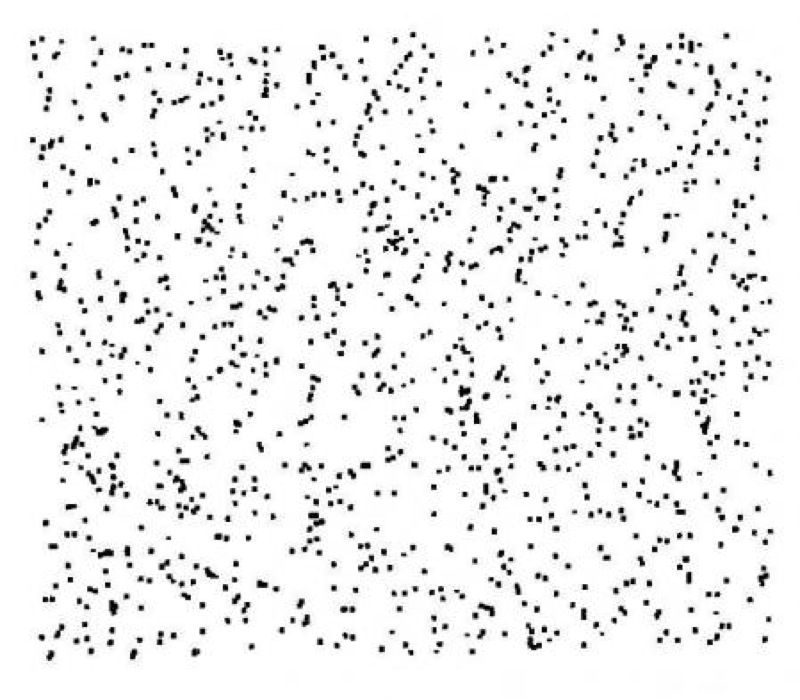
\includegraphics[width=0.618\textwidth]{pictures/pointa.jpg}}
\title{Stochastik}
\subtitle{Wahrscheinlichkeiten \& Kombinatorik}
\author{}
\date{}
\lowertitleback{

\includegraphics[height=1cm]{pictures/gymfmslerbermattlogo.eps}
\hfill%\copyright%
{\begin{tikzpicture}
  % Draw the rounded rectangle and clip the image to it
  \clip [rounded corners=5mm] (0,0) rectangle (1,1); % Adjust dimensions as needed
  \node at (0.5,0.5) {\includegraphics[width=1cm]{pictures/teacher_me_caricatur.png}}; % Adjust width and center image
\end{tikzpicture}}
}


\begin{document}

\clearpage

\appendix

\section{Kombinatorik}
\subsection{Problemstellungen}
\begin{itemize}
\item Warum wird den Schweizern der \glqq Schieber\grqq\ auf die Dauer nicht langweilig? Weil es
$$21\,452\,752\,266\,265\,320\,000$$
verschiedene Spiele dieser Art gibt!
\item Warum spielen jede Woche so viele Leute im deutschen Zahlenlotto \glqq 6 aus 49\grqq?
Weil sie nicht wissen, dass ihre Gewinnchance für sechs Richtige verschwindend klein ist, nämlich nur $1\div13\,983\,816$!
\item Warum verwenden gewöhnliche Bankräuber für das Öffnen eines Safes Schweissbrenner?
Weil sie viel zu viel Zeit bräuchten, sämtliche Kombinationen des Zahlenschlosses durchzuprobieren!
\end{itemize}

Mit diesen und ähnlichen Problemen beschäftigt sich die \definition{Kombinatorik}, ein Teilgebiet der Arithmetik. Sie untersucht, auf wie viele Arten bestimmte Objekte ausgewählt und wie diese Objekte angeordnet werden können. Wir wollen uns auf die Auswahl aus endlichen Mengen beschränken; Kombinatorik ist im wesentlichen finite Mathematik. Die zwei wichtigsten Probleme für die Kombinatorik sind:
\begin{itemize}
\item das \emph{Existenzproblem}: Welche Möglichkeiten gibt es, Elemente einer endlichen Menge nach bestimmten Bedingungen auszuwählen oder anzuordnen?
\item das \emph{Aufzählungsproblem}: Wie viele Möglichkeiten gibt es dafür insgesamt?
\end{itemize}

Dabei kann sich durchaus ergeben, dass unter den gestellten Bedingungen gar keine Lösung existiert. Bei praktischen Aufgaben stellt sich zudem oft die Frage, wie man die Lösungen am besten klassifizieren kann bzw. welche Lösung ein Optimum für bestimmte Zwecke darstellt.

Mit den folgenden fünf Aufgaben sollen zunächst die wesentlichen Aufgabentypen der Kombinatorik, die in der Schulmathematik ihren Platz gefunden haben, vorgestellt werden. Diese Aufgaben werden später auf ein gemeinsames Modell, das Urnenmodell, zurückgeführt.

\begin{uebenv}{torundsissi}
Wie viele verschiedene Buchstabenfolgen kann man mit den Buchstaben
\begin{enumerate}[a)]
\item \texttt{T, O, R}
\item \texttt{S, I, S, S, I}
\end{enumerate}
bilden, wenn jeweils alle Buchstaben zu verwenden sind?
\end{uebenv}

\begin{lsg}{torundsissi}
\begin{enumerate}[a)]
\item An der ersten drei Positionen kann man aus $3$ Buchstaben w\"ahlen, bei der n\"achsten noch aus $2$ und danach setzt man noch den \"ubrig gebliebenen Buchstaben; also kann dies auf $3\cdot2\cdot1=3!=6$ Arten geschehen.
\item Hier ist es kniffliger, da man gleichartige Buchstaben hat. Ich denke mir die gleichartigen durchnummeriert (z.B. $I_{1}, I_{2}$). Jetzt berechne ich die Kombinationen als h\"atte ich lauter Individuen. Abschliessend muss ich durch die Anzahl Kombinationsm\"oglichkeiten aller durchnummerierten, gleichartigen dividieren, da sie sich ja eigentlich nicht unterscheiden lassen. F\"ur \texttt{SISSI} gibt es also $\frac{5!}{2!\cdot3!}=10$ M\"oglichkeiten.
\end{enumerate}
\end{lsg}

\begin{uebenv}{totogoal}
Wie viele Prognosen können für die beiden ersten Fussballspiele eines Totozettels gegeben werden?
\begin{figure}
\begin{center}
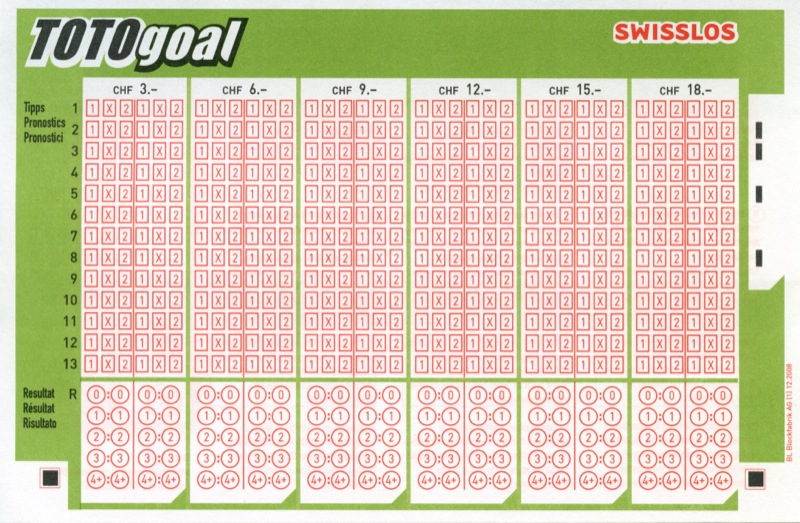
\includegraphics[width=0.618\textwidth]{pictures/TotoGoal}
\caption{TOTOgoal Tippspiel}
\end{center}
\end{figure}
\end{uebenv}

\begin{lsg}{totogoal}
Das sind $3\cdot3=9$.
\end{lsg}


\begin{uebenv}{apfelkuchen}
 Für eine kleine Apfelwähe lässt sich Frau Gschwind von ihrem Kaufmann, der die Sorten \emph{Gravensteiner} und \emph{Delicious} --- gemischt in einer grossen Kiste --- verkauft, vier beliebige Äpfel geben. Wie viele verschiedene Apfelwähen könnten so entstehen?
 \end{uebenv}

\begin{lsg}{apfelkuchen}
Das sind $5$. Ich stelle mir die vier \"Apfel (\faApple) in einer Reihe ausgelegt vor. Nun kann ich mit einer Trennwand die beiden Sorten aufteilen. Diese Trennwand kann ich an $5$ verschiedenen Stellen ($\_$) positionieren:
$\_\ \text{\faApple}\ \_\ \text{\faApple}\ \_\ \text{\faApple}\ \_\ \text{\faApple}\ \_$
\end{lsg}
  
 Aus der Mannigfaltigkeit der kombinatorischen Aufgaben seien hier noch erwähnt:
 \begin{itemize}
 \item In any calendar year how many Friday the thirteenths can there be? (Minimum: 1, Maximum: 3)
 \item Wie viele \glqq Gesichter\grqq\ hat der Zauberwürfel (Rubik's Cube)?\\ ($43\,252\,003\,274\,489\,856\,000$)
 \item Auf wie viele Arten lässt sich ein Franken in Kleingeld ($\unit[1]{Rp}$, $\unit[2]{Rp}$, $\unit[5]{Rp}$, $\unit[10]{Rp}$, $\unit[20]{Rp}$, $\unit[50]{Rp}$) umwechseln? (4562)
 \end{itemize}
 
 Aus den bisherigen Aufgaben mag der Eindruck entstehen, dass es sich bei der Kombinatorik um eine \glqq gehobene Unterhaltungsmathematik\grqq\ handelt. Tatsächlich gab es erst um 1900 ein erstes ernstzunehmendes Lehrbuch der Kombinatorik, das Lösungsmethoden für sämtliche klassische Aufgaben bereitstellte. Seit 1950 etwa ist die Kombinatorik zu einer anerkannten und selbständigen Disziplin innerhalb der Mathematik geworden. In anderen mathematischen Disziplinen (Wahrscheinlichkeitsrechnung, Zahlentheorie, Graphentheorie etc.), aber auch in anderen Wissenschaften (Linguistik, Biologie, Physik, Nachrichtentechnik etc.) tauchten immer mehr Probleme auf, die nur mit kombinatorischen Mitteln zu lösen waren. Insbesondere erlaubten seit 1950 die Computer ein experimentelles Arbeiten, das ganz neue Lösungswege eröffnete. Ein schönes Beispiel dazu ist der Beweis des Vierfarbensatzes. 1852 wurde folgendes Problem formuliert:
 \begin{quote}
Jede auf einem Stück Papier gezeichnete Landkarte lässt sich mit nur vier Farben so färben, dass niemals zwei aneinandergrenzende Länder dieselbe Farbe erhalten.
 \end{quote}
Erst 1976 konnte nach jahrelanger ständiger Verbesserung der Methoden mit 1200 Stunden Rechenzeit an drei Computern der Satz bewiesen werden.

\subsection{Summen- und Produktregel}
Will man die Anzahl der Schüler einer Schule ermitteln so könnte man an einem bestimmten Morgen jeder Schüler, der durch die Eingangstüre kommt, einzeln zählen. Einfacher wäre es, die einzelnen Klassenbestände zu ermitteln und zu addieren.
Die Idee ist folgende: Um die Anzahl der Elemente einer Menge $G$ zu ermitteln, ist es oft einfacher, diese Menge zuerst in elementfremde Teilmengen $A_1, A_2, A_3, \dots, A_r$ zu zerlegen und dann die entsprechenden Zahlen zu addieren.

\begin{csatz}[Summenregel]
$$\card(G)=\card(A_1)+\card(A_2)+\dots+\card(A_r)$$
wobei $A_i\cap A_j=\emptyset, i,j=1,2,\dots,r$.
\end{csatz}

\noindent\yinipar{E}\\[-1ex]
\textgoth{in Restaurant bietet Menus in vier Gängen an, die man nach freier Wahl zusammenstellen kann. Viel Vergnügen bei Ihrer Wahl aus drei Vorspeisen, zwei Zwischengängen, vier Hauptspeisen und drei Desserts.}

\begin{center}
  {\huge \textgoth{MENU}}\\[1ex]
  \Large
\textgoth{Feine Fenchelcrèmes:uppe\\
Indische Currys:uppe\\
Schildkrötens:uppe \glqq Lady Curzon\grqq\\
{\normalsize\ding{91}\quad\ding{91}\quad\ding{91}}\\
Schnecken nach Elsässer Art\\
Langustencocktail \glqq Nizza\grqq\\
{\normalsize\ding{91}\quad\ding{91}\quad\ding{91}}\\
Porterhous:e Steak\\
Flambierte Truthahnbrust\\
Seezunge \glqq Marguery\grqq\\
Aladins: Wunderpfanne\\
{\normalsize\ding{91}\quad\ding{91}\quad\ding{91}}\\
Eis:schale \glqq Blue Canary\grqq\\
Crèpes: à la pays:anne\\
Iris:h coffee}
 \end{center}
 
 \normalfont\normalsize
 
Nicht jede Zusammenstellung wird kulinarischen Regeln genügen, aber es gibt $3\cdot2\cdot4\cdot3=72$ verschiedene Menus.

Verallgemeinerung: Kann ein Vorgang auf $n_1$ verschiedene Arten ausgeführt werden, danach ein weiterer auf $n_2$ verschiedene Arten, dem folgend ein dritter auf $n_3$ verschiedene Arten, und so weiter, dann gibt es $n_1\cdot n_2\cdot n_3\cdot\dots\cdot n_k$ verschiedene Möglichkeiten, den so beschriebenen Gesamtvorgang auszuführen.

\begin{csatz}[Produktregel]
$$\text{Anzahl}=n_1\cdot n_2\cdot n_3\cdot\dots\cdot n_k$$
\end{csatz}

\begin{bem}
Zur Visualisierung kann ein Baumdiagramm gezeichnet werden.
\end{bem}

\marginnote{
\qrcode{
https://www.youtube.com/watch?v=8220w9uzGR0}
}

\begin{uebenv}{vierstellig}
Wie viele vierstellige Zahlen mit lauter ungeraden Ziffern gibt es?
\end{uebenv}

\begin{lsg}{vierstellig}
Pro Stelle hat man $5$ ungerade Ziffern zur Verf\"ugung, also gibt es $5^{4}=625$ M\"oglichkeiten.
\end{lsg}


\begin{uebenv}{kvkvk}
Wie viele \glqq Wörter\grqq\ der Form \texttt{KVKVK} (\texttt{K}: Konsonant, \texttt{V}: Vokal) gibt es, wenn ein Buchstabe \begin{enumerate}[a)]
\item mehrfach
\item nur einmal verwendet werden darf?
\end{enumerate}
\end{uebenv}

\begin{lsg}{kvkvk}
Es gibt $21$ Konsonanten und $5$ Vokale.
\begin{enumerate}[a)]
\item $21^{3}\cdot5^{2}=231\,525$
\item $21\cdot5\cdot20\cdot4\cdot19=159\,600$
\end{enumerate}
\end{lsg}

\begin{uebenv}{autonummer}
In der Schweiz enthalten die Nummernschilder der Autos in der Regel zwei Buchstaben (Kantonszeichen), denen sechs Ziffern folgen, wobei die erste nicht Null ist. Wie viele Schilder gibt es?
\end{uebenv}

\begin{lsg}{autonummer}
Es gibt theoretisch $26\cdot9\cdot10^{5}=23\,400\,000$ verschiedene Schilder.
\end{lsg}


\subsection{Permutationen}
In einer obigen Aufgabe hat man gesehen, dass die Buchstaben \texttt{T, O} und \texttt{R} auf sechs verschiedene Arten (\texttt{TOR, TRO, ORT, OTR, RTO, ROT}) angeordnet (permutiert) werden können. Auf die Anzahl 6 schliesst man mit der Produktregel: Für den ersten Buchstaben stehen drei Möglichkeiten (\texttt{T,O} oder \texttt{R}) zur Verfügung, für den zweiten bleiben noch zwei Möglichkeiten, für den dritten bleibt nur noch eine Möglichkeit. Insgesamt gibt es also $3\cdot2\cdot1=6$ verschiedene Möglichkeiten der Anordnung.
Allgemein gilt:

\begin{csatz}[Permutation]
Die Anzahl aller Permutationen von $n$ verschiedenen Elementen ist
$$P_n=n\cdot(n-1)\cdot(n-2)\cdot\dots\cdot3\cdot2\cdot1\stackrel{\text{Def.}}{=:}n!$$
\end{csatz}

\begin{bem}
$n!$ spricht man \glqq $n$ \definition{Fakult\"at}\grqq\ aus.
\end{bem}

\begin{bem}
Zwei Permutationen gelten als verschieden, wenn mindestens zwei Elemente nicht an der gleichen Stelle stehen.
\end{bem}

\begin{uebenv}{ausrufezeichen}
Berechne bzw. vereinfache:

\begin{enumerate}[a)]
\item $\frac{10!}{3!}$
\item $\frac{3\cdot4!}{4\cdot3!}$
\item $n(n-1)!$
\item $\frac{(n+3)!}{n!}\div\frac{(n+1)!}{(n-1)!}$
\end{enumerate}
\end{uebenv}

\begin{lsg}{ausrufezeichen}
\begin{enumerate}[a)]
\item $604\,800$
\item $3$
\item $n\cdot(n-1)!=n!$
\item $\frac{(n+3)!}{n!}\div\frac{(n+1)!}{(n-1)!}=\frac{(n+3)!(n-1)!}{n!(n+1)!}=\frac{(n+3)(n+2)}{n}$
\end{enumerate}
\end{lsg}


\begin{uebenv}{naturbuecher}
$3$ Physikbücher, $4$ Informatikbücher und $5$ Mathematikbücher sollen auf ein Regal gestellt werden. Auf wie viele Arten geht dies, wenn die Bücher des gleichen Fachgebiets nebeneinander stehen sollen und alle Bücher verschieden sind?
\end{uebenv}

\begin{lsg}{naturbuecher}
Die F\"acher kann man paketweise auf $3!$ Arten anordnen. Innerhalb dieser F\"acher sind dann insgesamt $3!\cdot4!\cdot5!$ Anordnungen m\"oglich. Das ergibt ein Total von sagenhaften $103\,680$ verschiedenen Anordnungen.
\end{lsg}


\begin{figure}[h]
\begin{center}
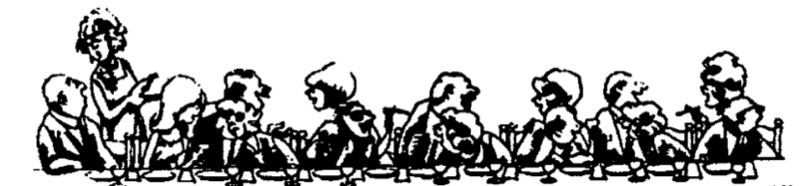
\includegraphics[width=0.8\textwidth]{pictures/seating}
\caption{\glqq Next time, let me handle the seating arrangements!\grqq}
\end{center}
\end{figure}
\begin{uebenv}{roundtable}
\ \\[-4ex]
\begin{enumerate}[a)]
\item Auf wie viel Arten können sich elf Personen in eine Reihe setzen?
\item Wie viele Möglichkeiten gibt es, wenn zwei Personen unbedingt nebeneinander sitzen wollen?
\item Löse (a) und (b) für die Sitzordnungen an einem runden Tisch.
\end{enumerate}
\end{uebenv}

\begin{lsg}{roundtable}
\begin{enumerate}[a)]
\item $11!\approx\unit[40]{Mio.}$
\item Die beiden Personen k\"onnen auf $2$ Arten nebeneinander sitzen. Nun kann dieses P\"archen sich zwischen und um die $9$ verbliebenen Personen setzen, die sich permutieren k\"onnen: $2!\cdot10\cdot 9!=7\,257\,600$.
\item $11!/11=10!=3\,628\,800$ und $10!/10\cdot2!=725\,760$
\end{enumerate}
\end{lsg}


Gegeben seien $n$ Elemente, von denen genau $k$ untereinander gleich sind. Diese $k$ gleichen Elemente werden für einen Moment mit Indizes versehen, so dass man sie voneinander unterscheiden kann. Die Anzahl aller Permutationen ist dann $n!$, wobei aber jeweils $k!$ Permutationen sich nur in den Stellungen der extra verschieden bezeichneten Elemente unterscheiden. Macht man die Indizierung rückgängig, so sind jeweils $k!$ Permutationen nicht mehr voneinander verschieden. Also ist in diesem Fall die Anzahl der Permutationen $\frac{n!}{k!}$.
Allgemein gilt:

\begin{csatz}[Permutation von k aus n]
Die Anzahl der Permutationen von $n$ Elementen, unter denen ein Element $k_1$-mal, ein zweites Element $k_2$-mal, ein drittes Element $k_3$-mal, \dots , ein $r$-tes Element $k_r$-mal vorkommt, ist
$$P_{n,k_1,\dots,k_r}=\frac{n!}{k_1!\cdot k_2!\cdot k_3!\cdot\dots\cdot k_r!}$$
\end{csatz}

\begin{uebenv}{mississippi}
Auf wie viele Arten kann man die Buchstaben von
\begin{enumerate}[a)]
\item \texttt{OTTO}
\item \texttt{MISSISSIPPI}
\item Deinen Namen für ein Anagramm permutieren?
\end{enumerate}
\end{uebenv}

\begin{lsg}{mississippi}
\begin{enumerate}[a)]
\item $\frac{4!}{2!\cdot2!}=6$
\item $\frac{11!}{(4!)^{2}\cdot2!}=34\,650$
\item \texttt{Jorma} $5!=120$
\end{enumerate}
\end{lsg}


\begin{uebenv}{schiffsfahnen}
Ein Signal kann durch sechs Fahnen, die untereinander hängen, gegeben werden. Wie viele verschiedene Signale kann man mit vier gleichen roten und zwei gleichen blauen Fahnen bilden?
\end{uebenv}

\begin{lsg}{schiffsfahnen}
$\frac{6!}{4!\cdot 2!}=15$
\end{lsg}


\subsection{Stichproben}
Die ersten Aufgaben aus dem Einführungskapitel sollen auf das Urnenmodell übertragen werden: In einer Urne sind $n$ Lose, die irgendwie gekennzeichnet sind. Aus dieser Urne werden $k$ Lose gezogen: eine \definition{Stichprobe} vom Umfang $k$.

Diese Ziehung kann auf vier verschiedene Arten erfolgen:
\begin{itemize}
\item[A] Jedes Los wird einzeln gezogen und nach einer Notiz wieder zurückgelegt. Es ergibt sich eine natürliche Ordnung; jedes Los kann mehrmals gezogen werden.

\definition{Geordnete Stichprobe mit Zurücklegen}.
\item[B]  Wie in A, jedoch wird das gezogene Los jeweils nicht zurückgelegt.

\definition{Geordnete Stichprobe ohne Zurücklegen}.
\item[C] Die $k$ Lose werden mit einem Griff gezogen, d.h. die natürliche Anordnung wie in A und B geht verloren.

\definition{Ungeordnete Stichprobe ohne Zurücklegen}.
\item[D] Wie in A, jedoch verzichtet man auf die sich ergebende Ordnung. Wenn in einer Urne von jedem Los mindestens $k$ Exemplare vorhanden sind, kann man auch wie in C mit einem Griff $k$ Lose ziehen.

\definition{Ungeordnete Stichprobe mit Zurücklegen}.
\end{itemize}

\subsubsection{Geordnete Stichprobe mit Zurücklegen}
Unmittelbar aus der Produktregel ergibt sich für die Anzahl der geordneten Stichproben mit Zurücklegen:
$$A_{n,k} = n\cdot n\cdot n\cdot\dots\cdot n=n^k$$
Bei der dualen Version werden nicht $k$ Lose aus einer Urne gezogen, sondern $k$ unterscheidbare Dinge auf $n$ unterscheidbare Urnen beliebig verteilt. Dazu gibt es $n\cdot n\cdot n\cdot\dots\cdot n=n^k$.

\begin{uebenv}{muenze}
Wie viele Ergebnisse sind möglich, wenn man
\begin{enumerate}[a)]
\item eine Münze
\item einen Würfel
\end{enumerate}
fünfmal wirft?
\end{uebenv}

\begin{lsg}{muenze}
\begin{enumerate}[a)]
\item $2^{5}=32$
\item $6^{5}=7776$
\end{enumerate}
\end{lsg}


\begin{uebenv}{safe}
Bei einem Safeschloss sind fünf Einstellungen einer Ziffer von 1 bis 9 möglich. Wie viel Zeit benötigt man, um alle Einstellungen auszuprobieren, wenn man für eine Einstellung durchschnittlich vier Sekunden braucht?
\end{uebenv}

\begin{lsg}{safe}
Man braucht $9^{5}\cdot4=\unit[236'196]{sec}$. Das sind ca. $65$ Stunden.
\end{lsg}


\subsubsection{Geordnete Stichprobe ohne Zurücklegen}
Auch in diesem Fall ergibt sich die Anzahl der geordneten Stichproben ohne Zurücklegen unmittelbar aus der Produktregel:
$$A_{n,k}=n\cdot(n-1)\cdot(n-2)\cdot\dots\cdot(n-k+1) = \frac{n!}{(n-k)!}$$
mit $k\leq n$.

Bei der dualen Version werden $k$ unterscheidbare Dinge so auf $n$ unterscheidbare Urnen verteilt, dass in jeder Urne höchstens ein Ding zu liegen kommt ($k\leq n$). Dazu gibt es $n\cdot(n-1)\cdot(n-2)\cdot\dots\cdot(n-k+1)$ Möglichkeiten.
Statt \glqq Urne\grqq\ sagt man bei dieser Version besser \glqq Platz\grqq.
Die Permutationen von $n$ verschiedenen Elementen sind ein Spezialfall der geordneten Stichprobe ohne Zurücklegen ($k=n$). Damit gibt es auch $n!$ verschiedene Möglichkeiten, $n$ voneinander verschiedene Dinge auf $n$ Plätze zu verteilen.

\begin{uebenv}{sprinter}
Acht Sprinter kämpfen bei den Olympischen Spielen um die Gold-, Silber- und Bronzemedaille. Auf wie viel Arten kann die Siegerehrung erfolgen?
\end{uebenv}

\begin{lsg}{sprinter}
$8\cdot7\cdot6=336$
\end{lsg}


\begin{uebenv}{sonderfall}
Wie sollte $0!$ definiert werden?
\end{uebenv}

\begin{lsg}{sonderfall}
Mit der Kombinatorik-Interpretation m\"ochte man $0$ Individuen permutieren. Dies geht auf $1$ Art, n\"amlich nicht. Ferner gilt $(n-k)!=\frac{n!}{n\cdot(n-1)\cdot\dots\cdot(n-k+1)}$, also im Falle $n=k$
$$0!=(n-n)!=\frac{n!}{n\cdot(n-1)\cdot\dots\cdot(n-n+1)}=\frac{n!}{n\cdot(n-1)\cdot\dots\cdot1}=\frac{n!}{n!}=1.$$
Somit setzt man $0!:=1$.
\end{lsg}


\subsubsection{Ungeordnete Stichprobe ohne Zurücklegen}
Für die Anzahl der ungeordneten Stichproben ohne Zurücklegen betrachte man noch einmal die Lösungen der Aufgaben aus dem Einführungskapitel.

Allgemein gilt: Jede der Stichproben vom Umfang $k$, die man mit einem Griff zieht, kann man auf $k!$ Arten ordnen. Nach dieser aufoktroyierten Ordnung hat man gerade den Fall der geordneten Stichproben ohne Zurücklegen. Deshalb gibt es $k!$ mal mehr geordnete als ungeordnete Stichproben.
Die Anzahl der ungeordneten Stichproben ohne Zurücklegen beträgt demnach:
$$A_{n,k}=\frac{n!}{(n-k)!}\div k!=\frac{n!}{k!(n-k)!}\stackrel{\text{Def.}}{=:}\binom{n}{k}$$
wobei $k\leq n$.

\begin{uebenv}{binomialkoeffizienten}

Zeige durch Rechnung
\begin{enumerate}[a)]
\item $\binom{n}{0}=\binom{n}{n}=1$
\item $\binom{n}{k}=\binom{n}{n-k}$
\item $\binom{n}{2}=\frac{n(n-1)}{2}$
\end{enumerate}
\end{uebenv}

\begin{lsg}{binomialkoeffizienten}
\begin{enumerate}[a)]
\item $\binom{n}{0}=\frac{n!}{0!\cdot n!}=\frac{n!}{1\cdot n!}=1$
\item $\binom{n}{k}=\frac{n!}{k!\cdot (n-k)!}=\frac{n!}{(n-k)!\cdot k!}=\frac{n!}{(n-k)!\cdot (n-(n-k))!}=\binom{n}{n-k}$
\item $\binom{n}{2}=\frac{n!}{2!\cdot(n-2)!}=\frac{n!}{2\cdot(n-2)!}=\frac{n(n-1)}{2}$
\end{enumerate}
\end{lsg}


\begin{uebenv}{delegation}
Aus zehn Schülern soll eine Delegation von vier Mitgliedern und innerhalb der Delegation ein Sprecher bestimmt werden. Auf wie viele Arten geht dies? Verallgemeinere auf $n$ Schüler und $k$ Delegationsmitglieder und leite so eine allgemeine Beziehung her.
\end{uebenv}

\begin{lsg}{delegation}
Aus $n$ Schüler die geforderten $k$ Delegationsmitglieder ausw\"ahlen kann man auf $\binom{n}{k}$ Arten. Aus den jeweils $k$ Delegierten gibt es $k$ m\"ogliche Sprecher: $k\cdot\binom{n}{k}$.
\end{lsg}


\begin{uebenv}{prost}
Wie viele Händedrücke gibt es, wenn sich $n$ Personen begrüssen und jeder jedem nur einmal die Hand gibt?
\end{uebenv}

\begin{lsg}{prost}
Es sind $\binom{n}{2}$ oder anders formuliert: Eine Person gr\"usst $(n-1)$ Leute. Da es $n$ Personen sind und egal. ob beispielsweise A B gr\"usst oder B A. gibt es $\frac{n(n-1)}{2}$ Begr\"ussungen.
\end{lsg}


\begin{uebenv}{jass}
Auf wie viele Arten kann man die 36 Jasskarten an

\begin{enumerate}[a)]
\item zwei
\item drei
\item vier
\end{enumerate}

Spieler verteilen?
\end{uebenv}

\begin{lsg}{jass}
\begin{enumerate}[a)]
\item $\binom{36}{18}\cdot\binom{18}{18}\approx9\cdot10^{9}$
\item $\binom{36}{12}\cdot\binom{24}{12}\approx3.4\cdot10^{15}$
\item $\binom{36}{9}\cdot\binom{27}{9}\cdot\binom{18}{9}\approx2.1\cdot10^{19}$
\end{enumerate}
\end{lsg}


\subsubsection{Ungeordnete Stichprobe mit Zurücklegen}
Für den schwierigsten Fall der ungeordneten Stichproben mit Zurücklegen formulieren wir die Anzahl-Apfelkuchen-Aufgabe ein wenig um: Auf wie viele Arten kann man \"Apfel aus der Menge $\set{\text{Delicious, Gravensteiner}}$ eine ungeordnete Stichprobe vom Umfang vier entnehmen?

Bezeichnet man mit $x_1\in\mN_0$ die Anzahl $D$ und mit $x_2\in\mN_0$ die Anzahl $G$, so muss die Anzahl der Lösungen der Gleichung $$x_1+x_2=4$$ ermittelt werden. Jede Lösung erhält man, wenn man in der Figur 1111 an geeigneter Stelle einen Trennstrich einsetzt. Zum Beispiel entspricht der Figur $$111|1$$ die Lösung drei Delicious und ein Gravensteiner. Für die Setzung des Trennstriches gibt es fünf Möglichkeiten, da der Trennstrich sowohl am Anfang als auch am Ende der Figur gesetzt werden kann. Es gibt demnach $\binom{5}{1}=5$ Stichproben.

Bevor wir auf $m$ Sorten und $k$ Apfel verallgemeinern, betrachten wir noch ein weiteres Beispiel mit $m=4$ und $k=10$. Die zugehörige Gleichung lautet: $$x_1+x_2+x_3+x_4=10$$ Aus der mit vertikalen Trennstrichen versehenen Figur $$111|11||11111$$ kann man die spezielle Lösung $x_1 = 3, x_2 = 2, x_3 = 0$ und $x_4 = 5$ ablesen. In diesem Beispiel hat man drei Trennstriche anzubringen. Die vollständige Figur besteht dann aus zehn Einsen und drei Trennstrichen. Man hat aus 13 Plätzen 10 Plätze für die Einsen oder 3 Plätze für die Trennstriche
auszuwählen, um alle gewünschten Stichproben zu erhalten. Dies geht auf $\binom{13}{10}=\binom{13}{3}=286$ Arten.

Im allgemeinen Fall sind $(m-1)$ Trennstriche anzubringen; die vollständige Figur besteht aus $k$ Einsen und $(m-1)$ Trennstriche. Schliesslich sind aus $k+(m-1)$ Plätzen deren $k$ für die Einsen oder deren $(m-1)$ für die Trennstriche auszuwählen.
Die Anzahl der ungeordneten Stichproben mit Zurücklegen beträgt also
$$A_{m,k}=\binom{m+k-1}{k}=\binom{m+k-1}{m-1}$$

\begin{uebenv}{zehnunbekannte}
Wie viele Lösungen hat die Gleichung
$$x_1+x_2+x_3+\dots+x_{10}=13\q (x\in\mN_0)?$$
\end{uebenv}

\begin{lsg}{zehnunbekannte}
$\binom{13+9}{9}=497\,420$
\end{lsg}

Bei der dualen Version sind $k$ ununterscheidbare Dinge in $m$ Urnen zu legen. Bezeichnet man die Dinge mit Einsen, so müssen in der Figur
$$11111\dots111$$
(m-1) Trennstriche als Markierungen für die Urnen gesetzt werden. Dazu gibt es, wie oben gezeigt,
$$\binom{m+k-1}{k}=\binom{m+k-1}{m-1}$$
Möglichkeiten.

\begin{uebenv}{parlamentssitze}
Auf wie viele Arten können 60 Parlamentssitze auf drei Parteien verteilt werden?
\end{uebenv}

\begin{lsg}{parlamentssitze}
$\binom{60+2}{2}=1891$
\end{lsg}


\begin{uebenv}{kaninchen}
Zehn ununterscheidbare Kaninchen sollen auf drei Käfige verteilt werden. Auf wie viele Arten geht dies, wenn
\begin{enumerate}[a)]
\item keine Einschränkungen vorgeschrieben sind
\item kein Käfig leer sein darf
\item kein Kaninchen allein und kein Käfig leer sein darf
\end{enumerate}
\end{uebenv}

\begin{lsg}{kaninchen}
\begin{enumerate}[a)]
\item $\binom{10+2}{2}=66$
\item Ich stecke in jeden K\"afig ein Kaninchen und verteile die restlichen $7$ nach belieben: $\binom{7+2}{2}=36$.
\item $\binom{4+2}{2}=15$
\end{enumerate}
\end{lsg}


\subsection{Übersicht}

\definecolor{lightyellow}{rgb}{1,1,0.8}
\definecolor{Gray}{gray}{0.9}
\begin{table}[h]
\large
\centering
\begin{tabular}{|c|c|c|} \hline
\rowcolor{Gray}\spaltenheight \emph{Stichproben} & mit Zurücklegen & ohne Zurücklegen\spaltensep\hline
\rowcolor{lightyellow}\spaltenheight geordnet & $n^k$ & $\frac{n!}{(n-k)!}$\spaltensep \hline
\rowcolor{Gray}\spaltenheight ungeordnet & $\binom{m+k-1}{m-1}$ & $\binom{n}{k}$\spaltensep \hline
\end{tabular}
\caption{Überblick der vier Fälle beim Ziehen}
\end{table}

\begin{figure}
\begin{center}
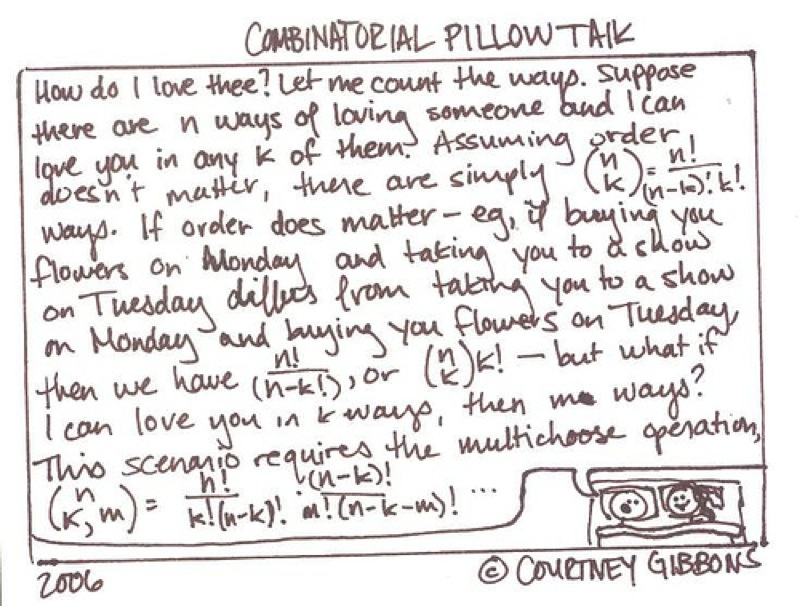
\includegraphics[width=0.8\textwidth]{pictures/pillowtalk}
\caption{Combinatorial Pillow-Talk}
\end{center}
\end{figure}

\subsection{Vermischte Aufgaben}

 \begin{uebenv}{dreisteller}
 Gegeben seien die Ziffern 1,2,3,4,5,6 und 7.
 \begin{enumerate}[a)]
 \item Wie viele dreistellige Zahlen mit verschiedenen
Ziffern lassen sich bilden?
 \end{enumerate}
 Wie viele davon sind
 \begin{enumerate}[a)]
 \addtocounter{enumi}{1}
 \item kleiner als 600
 \item kleiner als 600 und grösser als 300
 \item gerade
 \item ungerade
 \item durch 5 teilbar
 \item durch 25 teilbar?
 \end{enumerate}
 \end{uebenv}

\begin{lsg}{dreisteller}
\begin{enumerate}[a)]
\item $7\cdot6\cdot5=210$
\item $5\cdot6\cdot5=150$
\item $3\cdot6\cdot5=90$
\item $3\cdot6\cdot5=90$
\item $4\cdot6\cdot5=120$
\item $1\cdot6\cdot5=30$
\item $1\cdot2\cdot5=10$
\end{enumerate}
\end{lsg}

 
 \begin{uebenv}{obelix}
 Wie oft kann man im Schema \glqq Obelix\grqq\ ablesen?
 \begin{center}
 \ttfamily
 O\\
 B\q B\\
 E\q E\q E\\
 L\q L\q L\q L\\
 I\q I\q I\q I\q I\q\\
 X\q X\q X\q X\q X\q X
 \end{center}
 \end{uebenv}

\begin{lsg}{obelix}
$2^{5}=32$
\end{lsg}

\clearpage

\section{Der binomische Lehrsatz} \label{app:binomial}

\subsection{Motivation}

Von der Algebra her weis man, dass die Koeffizienten der Potenzen des Binoms $(a+b)$ in einem interessanten dreieckigen Zahlenschema übersichtlich dargestellt werden können.
Potenzen vom Typ $(a+b)$ sehen in der sukzessiven Entwicklung wie folgt aus:
\begin{align*}
(a+b)^0&=1\\
(a+b)^1&=a+b\\
(a+b)^2&=a^2+2ab+b^2\\
(a+b)^3&=a^3+3a^2b+3ab^2+b^3\\
\dots\q &= \q\dots\\
(a+b)^n&=a^n+na^{n-1}b+\dots+nab^{n-1}+b^n
\end{align*}

\subsection{Das Pascal'sche Dreieck}

Das Pascal'sche Dreieck gibt die Koeffizienten der zusammengefassten Summanden wieder:\\[-5ex]
\begin{center}
$$1$$
$$1\q1$$
$$1\q2\q1$$
$$1\q3\q3\q1$$
$$1\q4\q6\q4\q1$$
$$1\q5\q10\q10\q5\q1$$
$$\dots\qq\dots\qq\dots$$
$$1\q n\q\qq\dots\qq\q n\q1$$
\end{center}

\begin{bem}
Man beachte, dass die Exponenten der Summanden für $a$ von $n$ bis $0$ fallen, die von $b$ steigen von $0$ bis $n$.
\end{bem}

\begin{uebenv}{binom}
Berechne die ersten fünf Zeilen des folgenden Schemas:
\begin{center}
$$\binom{0}{0}$$
$$\binom{1}{0}\q\binom{1}{1}$$
$$\binom{2}{0}\q\binom{2}{1}\q\binom{2}{2}$$
$$\binom{3}{0}\q\binom{3}{1}\q\binom{3}{2}\q\binom{3}{3}$$\\[-1ex]
$$\dots\qq\dots\qq\dots$$\\[-2ex]
$$\binom{n}{0}\q\binom{n}{1}\qq\dots\qq\binom{n}{n-1}\q\binom{n}{n}$$
\end{center}
\end{uebenv}

\begin{lsg}{binom}
Man notiert das Pascal'sche Dreieck.
\end{lsg}

Aus der Lösung der Aufgabe erkennt man
\begin{csatz}[Pascal'sches Dreieck]
Berechnet man die $n$-te Potenz des Binoms $(a + b)$, so ist der
 Koeffizient von $a^{n-k}b^k$ gleich $\binom{n}{k}$ für $0\leq k\leq n$.
\end{csatz}
\begin{proof}[Beweis]
Um den Term mit $a^{n-k}b^k$ zu bekommen, muss man aus den $n$ Faktoren von $(a + b)^n = (a + b)(a + b)\dots(a + b)$ $k$ mal den Summanden $b$ auswählen. Aus den restlichen $n-k$ Faktoren wird dann nur noch der Summand $a$ berücksichtigt. Diese Auswahl kann auf $\binom{n}{k}$ Arten erfolgen.
\end{proof}

\begin{csatz}[Binomischer Lehrsatz]{}
\begin{align*}
(a+b)^n&=\binom{n}{0}a^n+\binom{n}{1}a^{n-1}b+\binom{n}{2}a^{n-2}b^2+\dots\\
&\dots+\binom{n}{n-1}ab^{n-1}+\binom{n}{n}b^n
\end{align*}
\end{csatz}

\begin{bem}
Die aus der Kombinatorik bekannten Zahlen $\binom{n}{k}$ nennt man deshalb auch \definition{Binomialkoeffizienten}.
\end{bem}

\begin{uebenv}{binom2}
\ \\[-4ex]
\begin{enumerate}[a)]
\item Welche Eigenschaft der Binomialkoeffizienten ergibt sich aus der Tatsache, dass jede Zeile im Pascal'schen Dreieck symmetrisch ist?
\item Zeige $$\binom{n}{k}+\binom{n}{k+1}=\binom{n+1}{k+1}$$ für $0\leq k\leq n-1$. Interpretiere diese Beziehung im Pascal'schen Dreieck.
\end{enumerate}
\end{uebenv}

\begin{lsg}{binom2}
\begin{enumerate}[a)]
\item $\binom{n}{k}=\binom{n}{n-k}$
\item Die Summe zweier benachbarter Binomialkoeffizienten ergibt den Binomialkoeffizienten eine Zeile weiter unten mittig.
\end{enumerate}
\end{lsg}

\clearpage

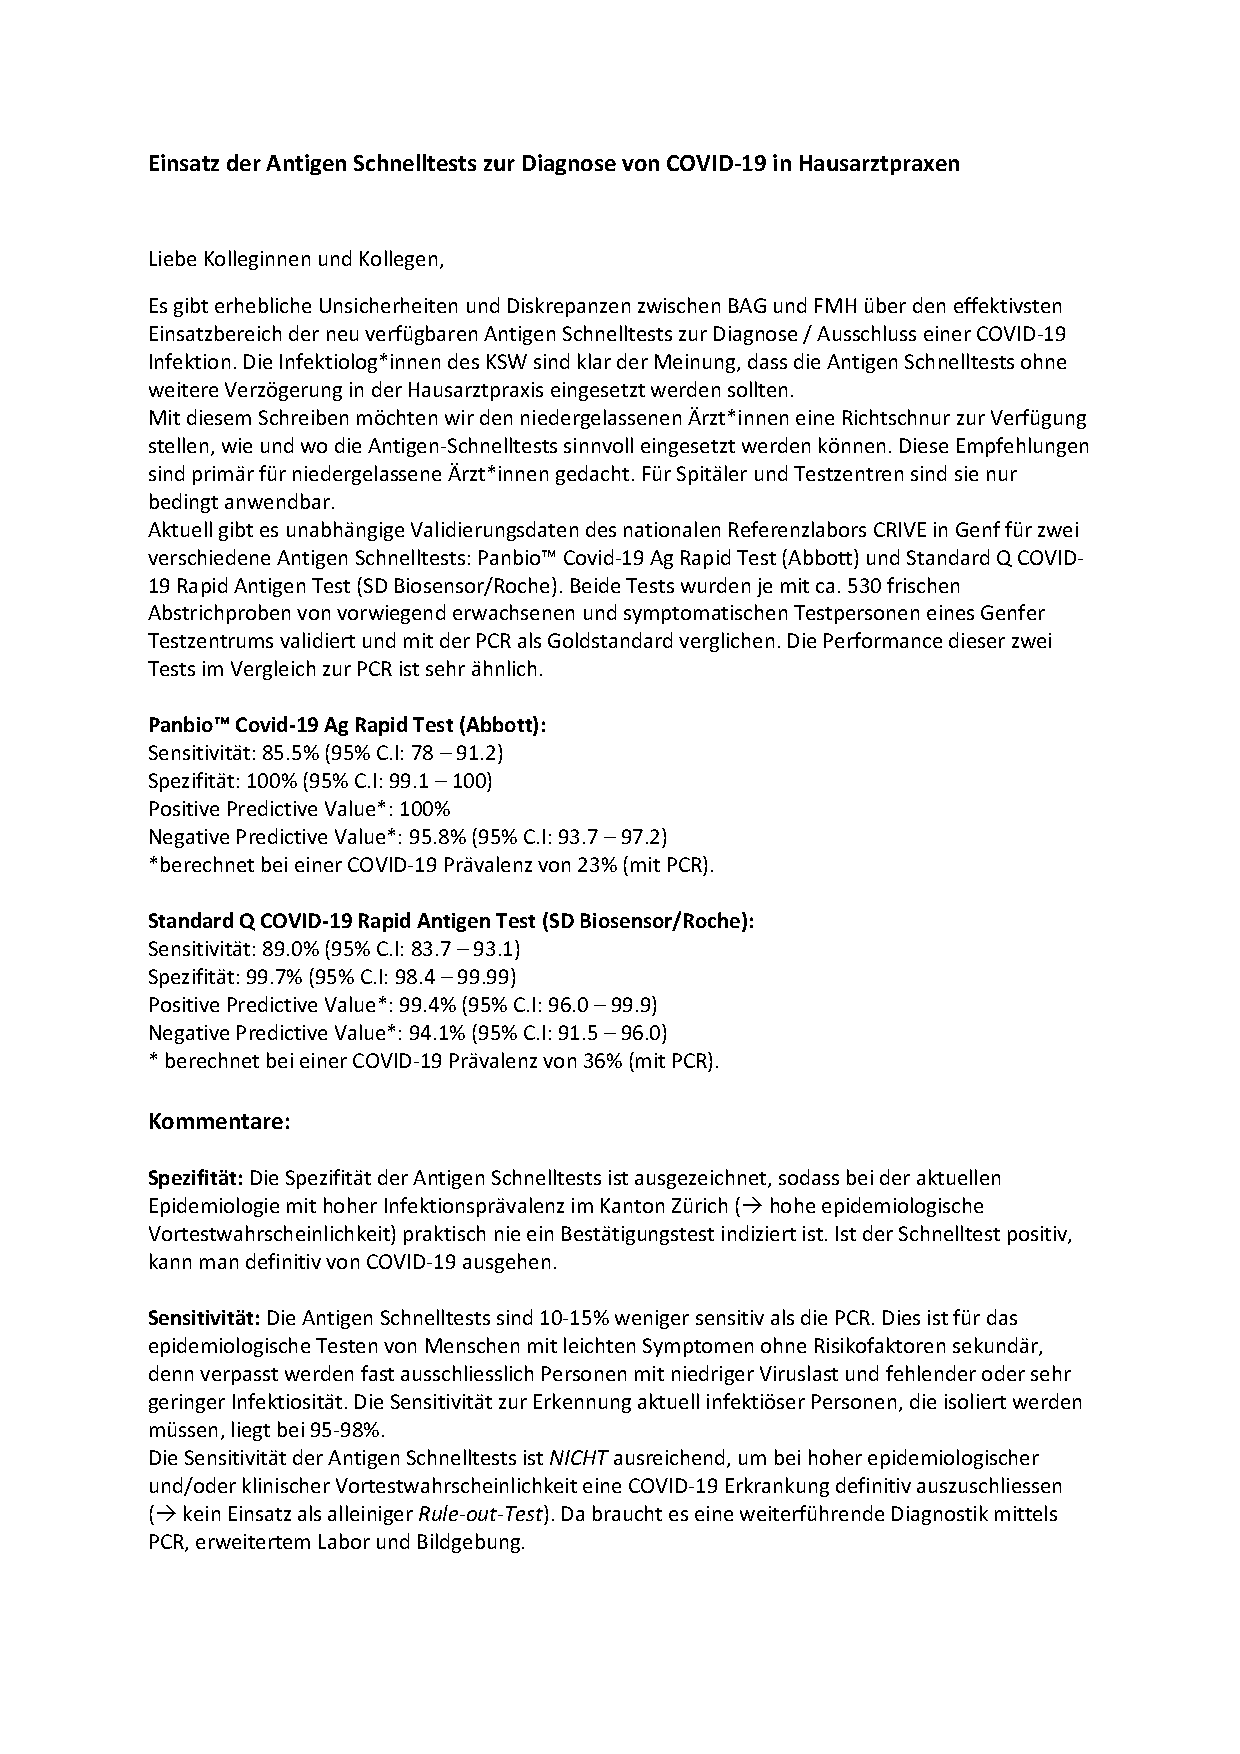
\includepdf[pages=1,pagecommand=\section{Aerzteinfo zu neuem CoVid-Schnelltest im Nov 2020\label{appendix:aerztecovid}},scale=0.85]{pictures/Aertzeinfocovid19.pdf}

\includepdf[pages=2-3,scale=0.85]{pictures/Aertzeinfocovid19.pdf}

\clearpage

\section{Gesetz der grossen Zahlen}

Was besagt das Gesetz der grossen Zahlen? Wikipedia sagt:

\begin{quote}
    In ihrer einfachsten Form besagen diese Sätze, dass sich die relative Häufigkeit eines Zufallsergebnisses in der Regel um die theoretische Wahrscheinlichkeit eines Zufallsergebnisses stabilisiert, wenn das zugrundeliegende Zufallsexperiment immer wieder unter denselben Voraussetzungen durchgeführt wird. Die häufig verwendete Formulierung, dass sich die relative Häufigkeit der Wahrscheinlichkeit \glqq immer mehr annähert\grqq\ ist dabei irreführend, da es auch bei einer großen Anzahl von Wiederholungen Ausreisser geben kann. Die Annäherung ist also nicht monoton.
\end{quote}

Das wollen wir uns in diesem Abschnitt genauer anschauen.

\subsection{Die Tschebyscheff'sche Ungleichung}

Wir brauchen für die folgende Argumentation die sogenannte Tschebyscheff-Ungleichung, die wir hier nicht streng beweisen wollen.

\begin{csatz}[Tschebyscheff'sche Ungleichung]{}
Sei $X$ eine Zufallsvariable mit Erwartungswert
$$\mu:=\mathrm{E}(X)$$
und endlicher Varianz
$$\sigma^2:=\mathrm{Var}(x).$$
Dann gilt für alle reellen Zahlen $k>0$:
$$P(\abs{X-\mu}\geq k)\leq \frac{\sigma^2}{k^2}.$$

Durch den Übergang zum komplementären Ereignis erhält man
$$P(\abs{X-\mu}< k)\geq 1-\frac{\sigma^2}{k^2}.$$
\end{csatz}

\begin{proof}
Als kleine Begründung (handwaving) betrachten wir für den diskreten Fall Instanzierungen $x_i, i\in I$ mit Wahrscheinlichkeit $p_i$. Was bedeutet für eine beliebige Zahl $k$ die Aussage $P(\abs{X-\mu}\geq k)$? Wir interessieren uns also für die Wahrscheinlichkeit, dass die Abweichung der Zufallsvariablen $X$ vom Erwartungswert $\mu$ grösser als $k$ ist. Nennen wir die Menge aller $i\in I$, so dass die Instanzierung der Zufallsvariablen grösser als $k$ ist
$$K:=\set{i\in I\,|\,\abs{x_i-\mu}\geq k}.$$
Wir lösen uns vom Betrag durch $(x_i-\mu)^2\geq k^2$ was äquivalent zu
$$\frac{(x_i-\mu)^2}{k^2}\geq 1.$$
Jetzt schätzen wir ab:

\begin{align*}
    P(\abs{X-\mu}\geq k) &= \sum_{i\in K}p_i\leq\sum_{i\in K}p_i\cdot\frac{(x_i-\mu)^2}{k^2}\leq\sum_{i\in I}p_i\cdot\frac{(x_i-\mu)^2}{k^2}\\
    &= \frac{1}{k^2}\cdot\sum_{i\in I}p_i(x_i-\mu)^2 = \frac{1}{k^2}\cdot\sigma^2
\end{align*}

Hieraus folgt unmittelbar
$$P(\abs{X-\mu}<k) \geq 1 - \frac{\sigma^2}{k^2}.$$
\end{proof}

\subsection{Herleitung}

Es gilt für eine Folge von i.i.d.\footnote{independent and identically distributed} Zufallsvariablen $X_1$, $X_2$, \dots. $X_n$ mit Erwartungswert $\mu$ und Varianz $\sigma^2$ für ihr arithmetisches Mittel (Mittelwert)
$$\bar{X}=\frac{X_1+\dots+X_n}{n}.$$
Beachte, dass $\bar{X}$ selbst wiederum eine Zufallsvariable ist. Es ist natürlich $\mathrm{E}(\bar{X})=\mu$ und für die Varianz gilt $\mathrm{Var}(\bar{X})=\frac{\sigma^2}{n}$, da für unabhängige Zufallsvariablen die Varianz linear ist. Somit folgt mit der Tschebyscheff'schen Ungleichung
$$P(\abs{\bar{X}-\mu}<k) \geq 1-\frac{\frac{\sigma^2}{n}}{k^2}.$$
was für $n\to\infty$ zu
$$\lim_{n\to\infty}P(\abs{\bar{X}-\mu}<k) \geq 1=1$$
wird. Das heisst: für eine grösser werdende Anzahl von i.i.d. Zufallsvariablen geht die Wahrscheinlichkeit, dass die Abweichung ihres Mittelwerts vom Erwartungswert kleiner als eine beliebige positive Zahl $k$ ist, gegen $100\%$.

\subsection{Konvergenz gegen die Wahrscheinlichkeit}

Beispielsweise gilt für Bernoulli-verteilte Zufallsvariablen $X_i$ mit Erfolgswahrscheinlichkeit $p$, dass ihr Mittelwert (relative Häufigkeit) gegen die Wahrscheinlichkeit konvergiert\footnote{Theorem von Bernoulli} (im Sinne von statistischer Konvergenz):
$$\bar{X}=\frac{X_1+\dots+X_n}{n}\stackrel{n\to\infty}{\longrightarrow}p.$$

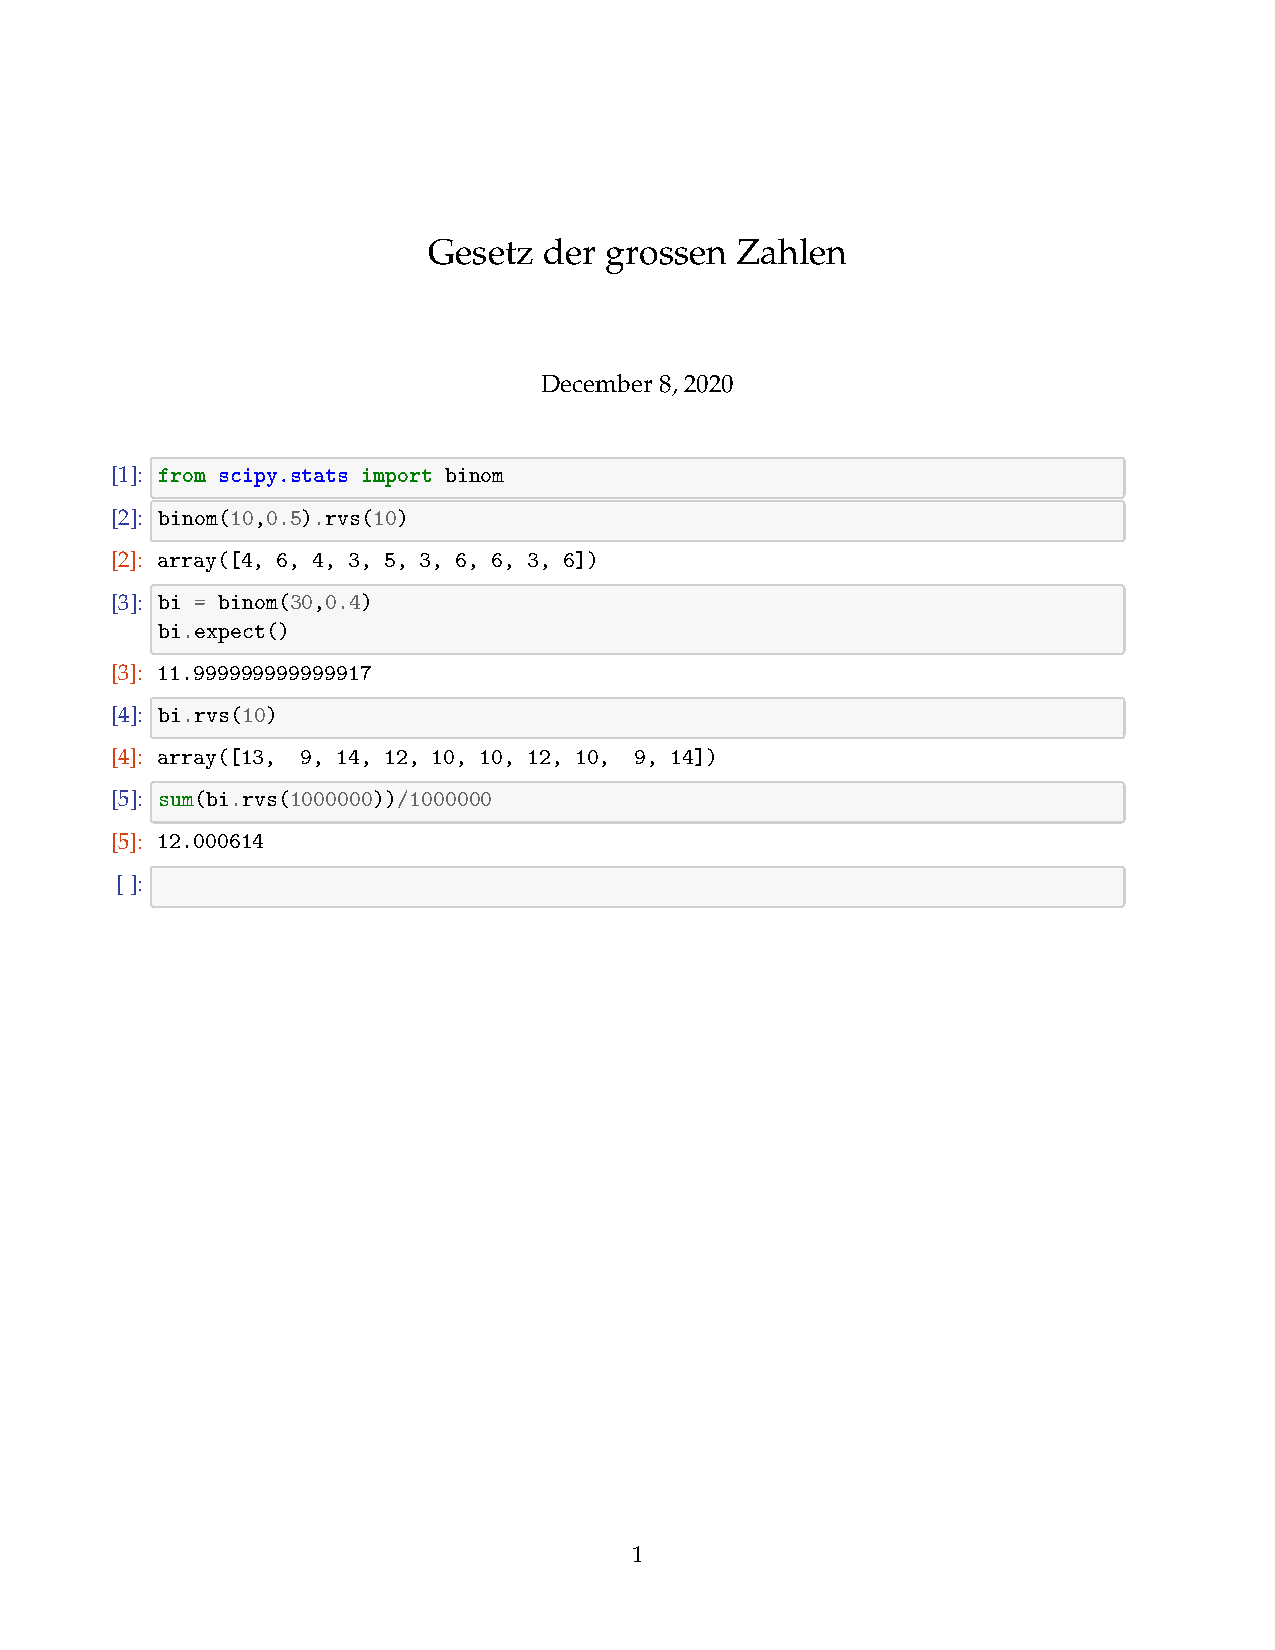
\includepdf[pages=1,pagecommand=\subsection{Konvergenz gegen die Wahrscheinlichkeiten in Messungen}]{pictures/gesetzzahlen.pdf}

\subsection{Missinterpretation des Gesetzes}

Ein Missverständnis, dem viele Leute erliegen, will ich noch ansprechen. Das Gesetz der grossen Zahlen besagt \emph{nicht}, dass man so was wie ausgleichende Gerechtigkeit hat, dass sich die Ergebnisse mit der Zeit ausgleichen. Nimm zum Beispiel eine faire Münze, werfe sie ein paar Mal und notiere dabei wie oft Kopf gezeigt wird. Dieses Verhältnis geht gegen $0.5$, wenn du die Anzahl der Würfe erhöhst (Gesetz der grossen Zahlen). Es wird aber nicht gesagt, dass sich Anzahl Kopf und Anzahl Zahl mit häufigerem Werfen ausgleichen werden. Betrachte dazu die Tabelle \ref{tab:grossezahlen} auf Seite \pageref{tab:grossezahlen}.

\begin{table}[]
\large
\centering
\begin{tabular}{|l||c|c|c|c|c|}
\hline
\rowcolor{Gray}\spaltenheight \# Würfe & $10$ & $100$ & $1\,000$ & \dots & $100\,000$\spaltensep \hline
\rowcolor{lightyellow}\spaltenheight \glqq Kopf\grqq & $4$ & $43$ & $440$ & \dots & $47\,000$ \spaltensep \hline
\rowcolor{Gray}\spaltenheight rel. Häufigkeit & $0.4$ & $0.43$ & $0.44$ & \dots & $0.47$\spaltensep \hline\hline
\rowcolor{lightyellow}\spaltenheight \glqq Zahl\grqq & $6$ & $57$ & $560$ & \dots & $53\,000$ \spaltensep \hline
\rowcolor{Gray}\spaltenheight $\Delta$ & $2$ & $14$ & $120$ & \dots & $6\,000$\spaltensep \hline
\end{tabular}
\caption{Münzwurf zur Illustration des Gesetzes der grossen Zahlen}\label{tab:grossezahlen}
\end{table}

\clearpage

\section{Alles ist Normalverteilt}

\subsection{Was ist eine Normalverteilung?}

Die Normal- oder Gauss-Verteilung\footnote{benannt nach Carl Friedrich Gauss} ist die wohl wichtigste Wahrscheinlichkeitsverteilungen. Die zugehörige Dichtefunktion kennt man auch unter dem Namen \definition{Gauss'sche Glockenkurve}.

\begin{figure}
    \centering
    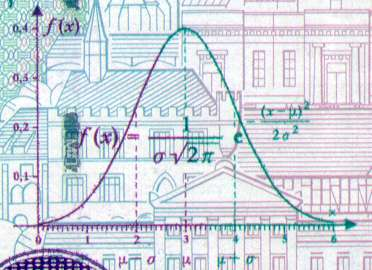
\includegraphics[width=0.382\textwidth]{pictures/gauss}
    \caption{Ausschnitt aus einer 10DM Note; findest du die Glockenkurve?}
    \label{fig:glockenkurve}
\end{figure}

In Wikipedia wird die Bedeutung der Normalverteilung folgendermassen beschrieben:
\begin{quote}
 Die besondere Bedeutung der Normalverteilung beruht unter anderem auf dem zentralen Grenzwertsatz, dem zufolge Verteilungen, die durch additive Überlagerung einer grossen Zahl von unabhängigen Einflüssen entstehen, unter schwachen Voraussetzungen annähernd normalverteilt sind.
 
 Die Abweichungen der Messwerte vieler natur-, wirtschafts- und ingenieurwissenschaftlicher Vorgänge vom Erwartungswert lassen sich durch die Normalverteilung (bei biologischen Prozessen oft logarithmische Normalverteilung) in sehr guter Näherung beschreiben (vor allem Prozesse, die in mehreren Faktoren unabhängig voneinander in verschiedene Richtungen wirken).
\end{quote}

\subsection{Die Standardnormalverteilung an einem Beispiel}

Sei $X_1$, $X_2$, $X_3$, \dots , $X_n$ eine Folge von i.i.d.\footnote{independent, identically distributed} Zufallsvariablen, deren Erwartungswert $\mu$ und Varianz $\sigma^2$ existieren.\footnote{Man kann sich für die Fortsetzung zum Beispiel vorstellen, dass diese $X_i$, $i\in\set{1,2,\dots,n}$ Messwerte seien.} Im Falle von beispielsweise $n=10$ ist der Mittelwert
$$\frac{X_1+\dots+X_{10}}{10}$$
selbst auch wieder eine Zufallsvariable mit einer gewissen Verteilung.

Für die folgende, theoretische Überlegung nehmen wir an, wir wüssten den Erwartungswert $\mu$. In der Praxis ist dies meist nicht der Fall und man versucht dieses $\mu$ so gut wie möglich zu schätzen. Wir setzen
$$Y_i:=X_i-\mu.$$
$Y_i$ ist also die Abweichung der Messung $X_i$ vom Erwartungswert. Man kann dies beispielsweise als Messungenauigkeit oder Rauschen interpretieren. Für den Erwartungswert von $Y_i$ folgt nun:
$$\mathrm{E}(Y_i)=\mathrm{E}(X_i-\mu)=\mathrm{E}(X_i)-\mathrm{E}(\mu)=\mathrm{E}(X_i)-\mu=0.$$
Die Varianz ändert sich natürlich bei der Verschiebung um $\mu$ nicht:
$$\mathrm{Var}(Y_i)=\mathrm{Var}(X_i)=\sigma^2.$$
Es folgt wegen der Unabhängigkeit der $Y_i$
$$\mathrm{Var}(Y_1+Y_2+\dots+Y_n)=\mathrm{Var}(Y_1)+\dots+\mathrm{Var}(Y_n)=n\cdot\sigma^2.$$
das heisst die Standardabweichung von $Y_1+\dots+Y_n$ ist
$$\sqrt{n\sigma^2}=\sqrt{n}\cdot\sigma.$$
Jetzt definieren wir uns eine neue Zufallsvariable
$$Z_n:=\frac{Y_1+\dots+Y_n}{\sqrt{n}\cdot\sigma}.$$
So ist $\mathrm{E}(Z_n)=0$ und $\mathrm{Var(Z_n)}=1$ (normiert). Diese neu definierte Zufallsvariable $Z_n$ konvergiert für grösser werdende $n$ immer gegen dieselbe Verteilung, nämlich der \definition{Standard-Normalverteilung}! Und dies unabhängig davon, welcher Verteilung die $X_i$, $i\in\set{1,\dots,n}$ unterliegen.

\subsection{Konvergenz gegen die Normalverteilung experimentell}

Es folgen ein paar Versuche unter verschiedenen Verteilungen. Das Programm \texttt{CRT(distr.nrandvals.miter)} macht dabei folgendes:
\begin{itemize}
    \item zufällig für eine gewisse Verteilung $n$ Werte generieren (rvs)
    \item Mittelwert zentrieren (expect)
    \item Standardabweichung normieren (std)
    \item mache das $m$ mal
    \item Plot als Histogramm (relative Häufigkeiten)
\end{itemize}

\clearpage

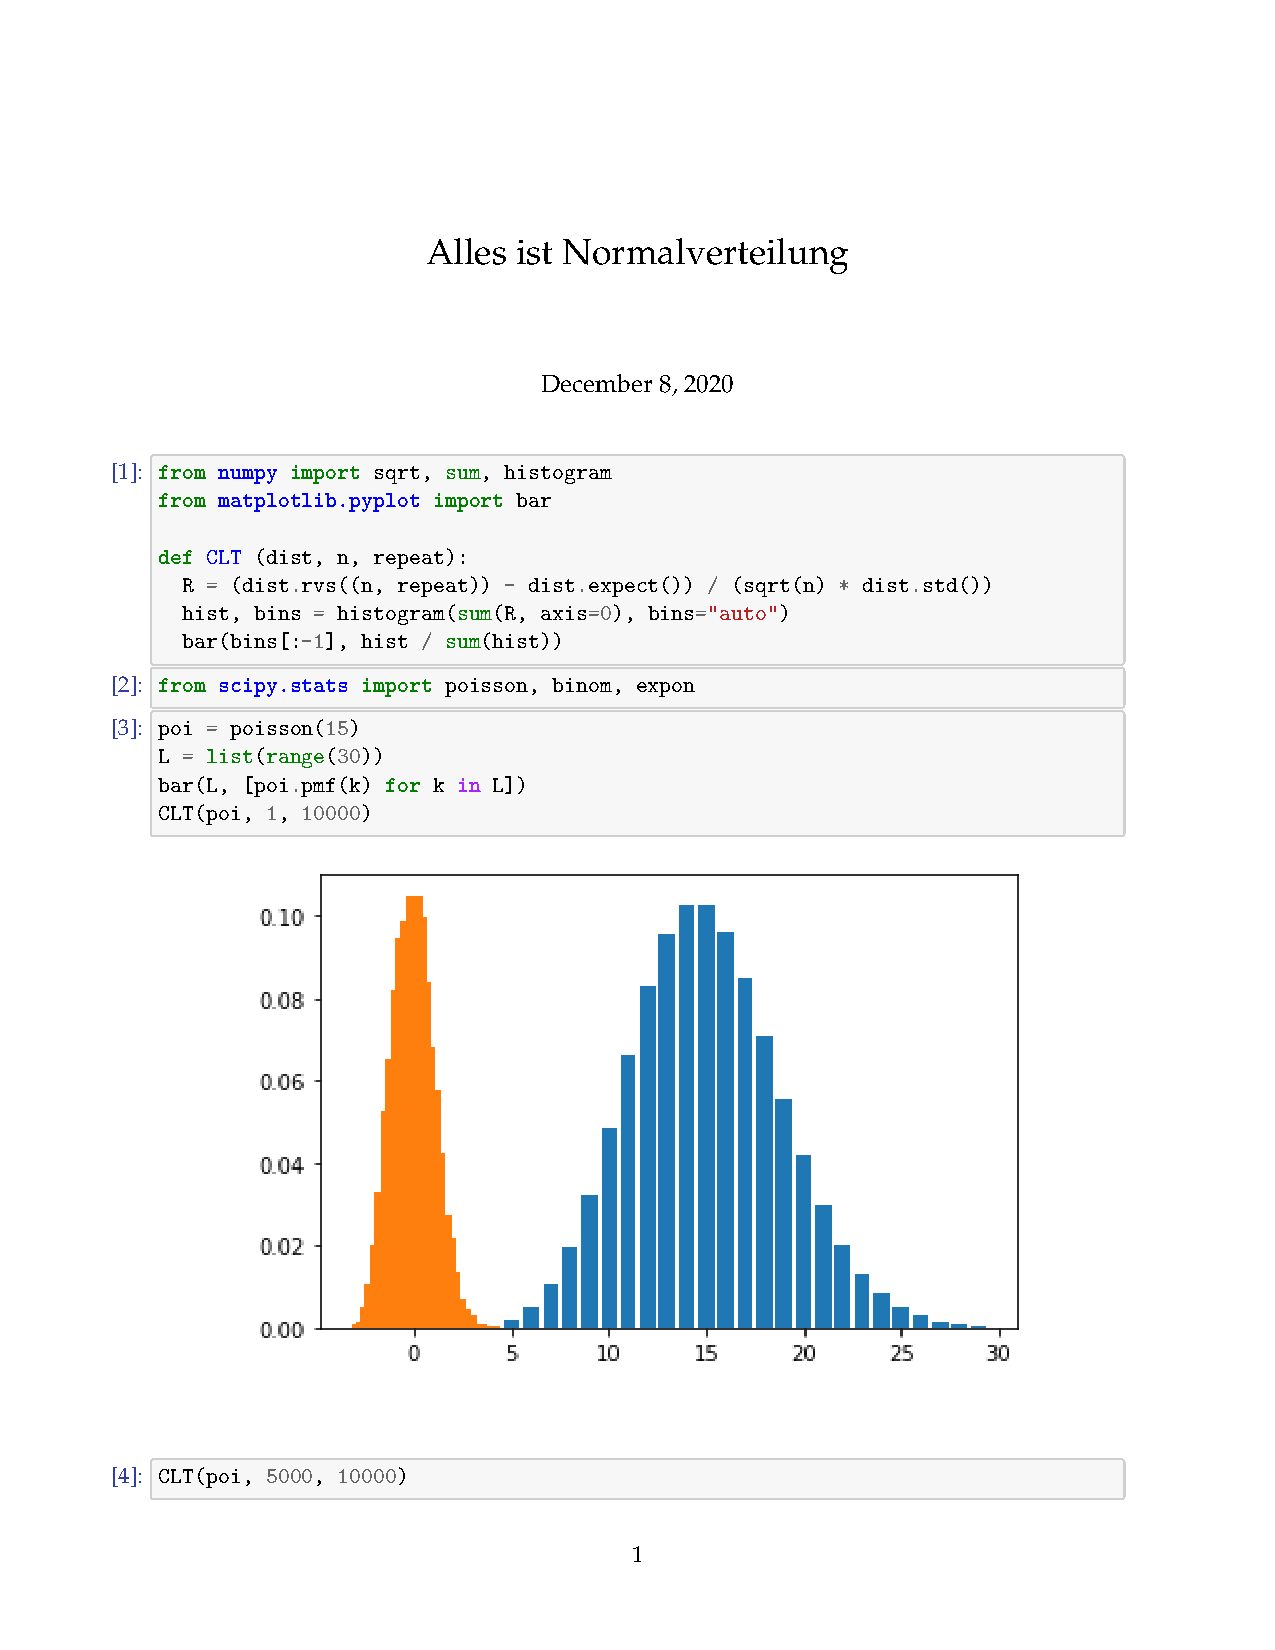
\includepdf[pages=1,pagecommand=\subsection{Verschiedene Verteilungen normiert}]{pictures/allesnorm.pdf}
\includepdf[pages=2-5]{pictures/allesnorm.pdf}

\clearpage

Man sieht, dass für jede der getesteten Verteilung eine zur unten abgebildeten Funktion ähnliche Kurve resultiert.

\begin{figure}
    \centering
\begin{tikzpicture}
\begin{axis}[
    axis lines = left,
    xlabel = $x$,
    ylabel = {$f(x)$},
]
%Below the red parabola is defined
\addplot [
    domain=-4:4, 
    samples=100, 
    color=red,
]
{exp(-x*x)};
\addlegendentry{$\mathrm{e}^{-x^2}$}
%Here the blue parabloa is defined
\addplot [
    domain=-4:4, 
    samples=100, 
    color=blue,
    ]
    {1/(2*3.14159)^0.5*exp(-0.5*x*x)};
\addlegendentry{$\frac{1}{\sqrt{2\pi}}\cdot e^{-\frac{x^2}{2}}$}

\end{axis}
\end{tikzpicture}
\caption{Glockenkurve und Standard-Normalverteilung}
\end{figure}

Grundsätzlich hat der Graph der Funktion
$$f(x)=e^{-x^2}$$
die Form einer Glockenkurve. Soll damit aber eine Wahrscheinlichkeitsverteilung abgebildet werden, so muss die Fläche unter $f$ $1$ sein. Speziell für den Erwartungswert $0$ und die Standardabweichung/Varianz $1$ findet man die sogenannte \definition{Standard-Normalverteilung}
$$\mathcal{N}(0,1)=\frac{1}{\sqrt{2\pi}}\cdot e^{-\frac{x^2}{2}}.$$
In der Praxis möchte man noch die Parameter $\mu$ (Erwartungswert) und $\sigma$ (Standardabweichung) einstellen können. Dies führt zur Darstellung der \emph{Normalverteilungsdichtefunktion} mit Erwartungswert $\mu$ und Standardabweichung $\sigma$:
$$\mathcal{N}(\mu,\sigma):=\frac{1}{\sqrt{2\pi\sigma^2}}\cdot e^{-\frac{(x-\mu)^2}{2\sigma^2}}.$$

\begin{uebenv}{}
Als Repetition könnte man an dieser Stelle Extrema und Wendestellen von $\mathcal{N}(\mu,\sigma)$ bestimmen; falls nicht bereits geschehen.
\end{uebenv}

Die Verteilungsfunktion
$$\Phi(x):=\frac{1}{\sqrt{2\pi}}\cdot\int_{-\infty}^{x} e^{-\frac{t^2}{2}}\,\mathrm{d}t$$
besitzt keine geschlossene Stammfunktion, weshalb man auf Tabellen zurückgreift. Wie oben gesehen kann man aber jede Zufallsvariable $X$ durch die Transformation zu $Z$ normieren, so dass nur die Standard-Normalverteilungsfunktion tabelliert werden muss. Siehe dazu die Tabelle \ref{tab:stddev} auf Seite \pageref{tab:stddev}. Um diese zu benutzen normiert man die normalverteilte Zufallsvariable $X$ zu $Z=\frac{X-\mu_{X}}{\sigma_{X}}$. Will man beispielsweise $P(x_{1}\leq X\leq x_{2})$ eruieren, so normiert man zu $P\left(\frac{x_{1}-\mu_{X}}{\sigma_{X}}\leq\frac{X-\mu_{X}}{\sigma_{X}}\leq \frac{x_{2}-\mu_{X}}{\sigma_{X}}\right)=P(z_{1}\leq Z\leq z_{2})$ und liest dann den $\Phi$-Wert aus der Tabelle.

\subsection{Der zentrale Grenzwertsatz}

Der zentrale Grenzwertsatz (von \textsc{Lindeberg-Lévy}) ist ein bedeutendes Resultat der Wahrscheinlichkeitstheorie. Er liefert die Begründung für das Phänomen, dass sich bei der additiven Überlagerung vieler unabhängiger Zufallseffekte zumindest approximativ eine Normalverteilung ergibt, wenn keiner der einzelnen Effekte einen dominierenden Einfluss auf die Varianz hat. Die in diesem wahrscheinlichkeitstheoretischen Sinne zu verstehende Konvergenz ist mit unseren Bezeichnungen die Gleichung
$$\lim_{n\to\infty} P(Z_n\leq x)=\Phi(x)$$
für beliebiges $x\in\mathbb{R}$.
Die zu den $Z_n$ gehörende Verteilungsfunktion wird also mit wachsendem $n$ durch die Normalverteilung approximiert.

\clearpage

\begin{table}[]
\centering
\caption{Standardnormalverteilungstabelle $\Phi(z)$}
\label{tab:stddev}
\scalebox{0.75}{
\begin{tabular}{l|llllllllll}
\rowcolor{Gray}\spaltenheight $z$   & 0.00       & 0.01    & 0.02    & 0.03    & 0.04    & 0.05    & 0.06    & 0.07    & 0.08    & 0.09    \\ \hline
\rowcolor{lightyellow}\spaltenheight 0.0   & 0.5     & 0.50399 & 0.50798 & 0.51197 & 0.51595 & 0.51994 & 0.52392 & 0.5279  & 0.53188 & 0.53586 \\
\rowcolor{Gray}\spaltenheight 0.1 & 0.53983 & 0.5438  & 0.54776 & 0.55172 & 0.55567 & 0.55962 & 0.56356 & 0.56749 & 0.57142 & 0.57535 \\
\rowcolor{lightyellow}\spaltenheight 0.2 & 0.57926 & 0.58317 & 0.58706 & 0.59095 & 0.59483 & 0.59871 & 0.60257 & 0.60642 & 0.61026 & 0.61409 \\
\rowcolor{Gray}\spaltenheight 0.3 & 0.61791 & 0.62172 & 0.62552 & 0.6293  & 0.63307 & 0.63683 & 0.64058 & 0.64431 & 0.64803 & 0.65173 \\
\rowcolor{lightyellow}\spaltenheight 0.4 & 0.65542 & 0.6591  & 0.66276 & 0.6664  & 0.67003 & 0.67364 & 0.67724 & 0.68082 & 0.68439 & 0.68793 \\
\rowcolor{Gray}\spaltenheight 0.5 & 0.69146 & 0.69497 & 0.69847 & 0.70194 & 0.7054  & 0.70884 & 0.71226 & 0.71566 & 0.71904 & 0.7224  \\
\rowcolor{lightyellow}\spaltenheight 0.6 & 0.72575 & 0.72907 & 0.73237 & 0.73565 & 0.73891 & 0.74215 & 0.74537 & 0.74857 & 0.75175 & 0.7549  \\
\rowcolor{Gray}\spaltenheight 0.7 & 0.75804 & 0.76115 & 0.76424 & 0.7673  & 0.77035 & 0.77337 & 0.77637 & 0.77935 & 0.7823  & 0.78524 \\
\rowcolor{lightyellow}\spaltenheight 0.8 & 0.78814 & 0.79103 & 0.79389 & 0.79673 & 0.79955 & 0.80234 & 0.80511 & 0.80785 & 0.81057 & 0.81327 \\
\rowcolor{Gray}\spaltenheight 0.9 & 0.81594 & 0.81859 & 0.82121 & 0.82381 & 0.82639 & 0.82894 & 0.83147 & 0.83398 & 0.83646 & 0.83891 \\
\rowcolor{lightyellow}\spaltenheight 1.0   & 0.84134 & 0.84375 & 0.84614 & 0.84849 & 0.85083 & 0.85314 & 0.85543 & 0.85769 & 0.85993 & 0.86214 \\
\rowcolor{Gray}\spaltenheight 1.1 & 0.86433 & 0.8665  & 0.86864 & 0.87076 & 0.87286 & 0.87493 & 0.87698 & 0.879   & 0.881   & 0.88298 \\
\rowcolor{lightyellow}\spaltenheight 1.2 & 0.88493 & 0.88686 & 0.88877 & 0.89065 & 0.89251 & 0.89435 & 0.89617 & 0.89796 & 0.89973 & 0.90147 \\
\rowcolor{Gray}\spaltenheight 1.3 & 0.9032  & 0.9049  & 0.90658 & 0.90824 & 0.90988 & 0.91149 & 0.91309 & 0.91466 & 0.91621 & 0.91774 \\
\rowcolor{lightyellow}\spaltenheight 1.4 & 0.91924 & 0.92073 & 0.9222  & 0.92364 & 0.92507 & 0.92647 & 0.92785 & 0.92922 & 0.93056 & 0.93189 \\
\rowcolor{Gray}\spaltenheight 1.5 & 0.93319 & 0.93448 & 0.93574 & 0.93699 & 0.93822 & 0.93943 & 0.94062 & 0.94179 & 0.94295 & 0.94408 \\
\rowcolor{lightyellow}\spaltenheight 1.6 & 0.9452  & 0.9463  & 0.94738 & 0.94845 & 0.9495  & 0.95053 & 0.95154 & 0.95254 & 0.95352 & 0.95449 \\
\rowcolor{Gray}\spaltenheight 1.7 & 0.95543 & 0.95637 & 0.95728 & 0.95818 & 0.95907 & 0.95994 & 0.9608  & 0.96164 & 0.96246 & 0.96327 \\
\rowcolor{lightyellow}\spaltenheight 1.8 & 0.96407 & 0.96485 & 0.96562 & 0.96638 & 0.96712 & 0.96784 & 0.96856 & 0.96926 & 0.96995 & 0.97062 \\
\rowcolor{Gray}\spaltenheight 1.9 & 0.97128 & 0.97193 & 0.97257 & 0.9732  & 0.97381 & 0.97441 & 0.975   & 0.97558 & 0.97615 & 0.9767  \\
\rowcolor{lightyellow}\spaltenheight 2.0   & 0.97725 & 0.97778 & 0.97831 & 0.97882 & 0.97932 & 0.97982 & 0.9803  & 0.98077 & 0.98124 & 0.98169 \\
\rowcolor{Gray}\spaltenheight 2.1 & 0.98214 & 0.98257 & 0.983   & 0.98341 & 0.98382 & 0.98422 & 0.98461 & 0.985   & 0.98537 & 0.98574 \\
\rowcolor{lightyellow}\spaltenheight 2.2 & 0.9861  & 0.98645 & 0.98679 & 0.98713 & 0.98745 & 0.98778 & 0.98809 & 0.9884  & 0.9887  & 0.98899 \\
\rowcolor{Gray}\spaltenheight 2.3 & 0.98928 & 0.98956 & 0.98983 & 0.9901  & 0.99036 & 0.99061 & 0.99086 & 0.99111 & 0.99134 & 0.99158 \\
\rowcolor{lightyellow}\spaltenheight 2.4 & 0.9918  & 0.99202 & 0.99224 & 0.99245 & 0.99266 & 0.99286 & 0.99305 & 0.99324 & 0.99343 & 0.99361 \\
\rowcolor{Gray}\spaltenheight 2.5 & 0.99379 & 0.99396 & 0.99413 & 0.9943  & 0.99446 & 0.99461 & 0.99477 & 0.99492 & 0.99506 & 0.9952  \\
\rowcolor{lightyellow}\spaltenheight 2.6 & 0.99534 & 0.99547 & 0.9956  & 0.99573 & 0.99585 & 0.99598 & 0.99609 & 0.99621 & 0.99632 & 0.99643 \\
\rowcolor{Gray}\spaltenheight 2.7 & 0.99653 & 0.99664 & 0.99674 & 0.99683 & 0.99693 & 0.99702 & 0.99711 & 0.9972  & 0.99728 & 0.99736 \\
\rowcolor{lightyellow}\spaltenheight 2.8 & 0.99744 & 0.99752 & 0.9976  & 0.99767 & 0.99774 & 0.99781 & 0.99788 & 0.99795 & 0.99801 & 0.99807 \\
\rowcolor{Gray}\spaltenheight 2.9 & 0.99813 & 0.99819 & 0.99825 & 0.99831 & 0.99836 & 0.99841 & 0.99846 & 0.99851 & 0.99856 & 0.99861 \\
\rowcolor{lightyellow}\spaltenheight 3.0   & 0.99865 & 0.99869 & 0.99874 & 0.99878 & 0.99882 & 0.99886 & 0.99889 & 0.99893 & 0.99896 & 0.999   \\
\rowcolor{Gray}\spaltenheight 3.1 & 0.99903 & 0.99906 & 0.9991  & 0.99913 & 0.99916 & 0.99918 & 0.99921 & 0.99924 & 0.99926 & 0.99929 \\
\rowcolor{lightyellow}\spaltenheight 3.2 & 0.99931 & 0.99934 & 0.99936 & 0.99938 & 0.9994  & 0.99942 & 0.99944 & 0.99946 & 0.99948 & 0.9995  \\
\rowcolor{Gray}\spaltenheight 3.3 & 0.99952 & 0.99953 & 0.99955 & 0.99957 & 0.99958 & 0.9996  & 0.99961 & 0.99962 & 0.99964 & 0.99965 \\
\rowcolor{lightyellow}\spaltenheight 3.4 & 0.99966 & 0.99968 & 0.99969 & 0.9997  & 0.99971 & 0.99972 & 0.99973 & 0.99974 & 0.99975 & 0.99976 \\
\rowcolor{Gray}\spaltenheight 3.5 & 0.99977 & 0.99978 & 0.99978 & 0.99979 & 0.9998  & 0.99981 & 0.99981 & 0.99982 & 0.99983 & 0.99983 \\
\rowcolor{lightyellow}\spaltenheight 3.6 & 0.99984 & 0.99985 & 0.99985 & 0.99986 & 0.99986 & 0.99987 & 0.99987 & 0.99988 & 0.99988 & 0.99989 \\
\rowcolor{Gray}\spaltenheight 3.7 & 0.99989 & 0.9999  & 0.9999  & 0.9999  & 0.99991 & 0.99991 & 0.99992 & 0.99992 & 0.99992 & 0.99992 \\
\rowcolor{lightyellow}\spaltenheight 3.8 & 0.99993 & 0.99993 & 0.99993 & 0.99994 & 0.99994 & 0.99994 & 0.99994 & 0.99995 & 0.99995 & 0.99995 \\
\rowcolor{Gray}\spaltenheight 3.9 & 0.99995 & 0.99995 & 0.99996 & 0.99996 & 0.99996 & 0.99996 & 0.99996 & 0.99996 & 0.99997 & 0.99997 \\
\rowcolor{lightyellow}\spaltenheight 4.0   & 0.99997 & 0.99997 & 0.99997 & 0.99997 & 0.99997 & 0.99997 & 0.99998 & 0.99998 & 0.99998 & 0.99998
\end{tabular}
}
\end{table}


\cleardoublepage
\listoffigures
\listoftables
%\newpage
%\nocite{*}
%\bibliographystyle{plain}
%\bibliography{preamble/literaturgoogle}
\end{document}